
\chapter{网页结构相似度计算与聚类}
\label{chap:cluster}
\section{基于最长公共子序列的网页距离计算}
\label{sec:lcs}
我们将DOM Tree的结构相似度转化成经过预处理模块得到的新的序列的相似度。这里,我们
将采用经典的最长公共子序列的方法计算两个序列的相似度。

假设经过预处理模块,文档$D_1,D_2$分别被转化为序列$S_1,S_2$,长度分别
为$len_1,len_2$,定义一个大小为$(len_1+1) * len(_2+1)$的二维表$T$,表的某个位
置$t(i + 1,j + 1),i,j >= 0$表示$S_1$的前$i$个元素组成的子序列和$S_2$前$j$个元素组
成的子序列的最长公共子序列长度。$T$的第一行和第一列的所有元素初始为0。根据$T$的定
义,我们只要计算出$T$中$t(len_1+1, len_2+1)$位置的值即可得到$S_1$和$S_2$的最长公
共子序列长度。

计算表格$T$我们有以下的递推公式:
\begin{eqnarray}
  \label{cluster:eqn:lcs}
  t(i)(j) =
  \begin{cases}
    0 & i = 0,\: j = 0\\
    t(i-1)(j-1) + 1 & i,\: j > 0, x_i=y_j\\
    \max(t(i)(j-1), t(i-1)(j)) & i, j > 0,\: x_i \ne y_j
  \end{cases}
\end{eqnarray}
$x_i$和$y_j$分别表示$S_1$的第$i$个元素和$S_2$的第$j$个元素。在以上递推过程中,我
们还可以同时记录每个位置的值是由哪个位置的值计算得到的,这样就可以通过回溯得到两
个序列的最长公共子序列了,记为$lcs(S_1,S_2)$。

得到了最长公共子序列的长度$|lcs(S_1,S_2)|$以后,文档$D_1$和$D_2$的相似度定义为:
\[
Sim(D_1,D_2)=\frac{|lcs(S_1,S_2)|}{\max(|S_1|,|S_2|)}
\]
\section{算法优化与改进}
\label{sec:optimize}
\subsection{优化和改进的动机}
前面给出的最长公共子序列的算法非常简单,然而,为了可以进行聚类,我们至少需要对文
档集合中每两个文档之间计算一次结构相似度。由于我们实验的数据量很大,即使进行离线
处理,如果不做优化的话,时间上也无法承受。

假设我们目前实现的计算最长公共子序列的算法运行一次平均需要$0.001s$,文档集合大小
为$60000$,在单线程的情况下,计算一次全部文档两两之间结构相似度的时间大约为:
\[
\frac{60000^2}{2 * 3600}*0.001=500h
\]

$500h$大约是21天左右,对于我们的实验来说,这个时间是不可承受的。

因为最长公共子序列的计算也是我们后续模板抽取工作的一个基础,除了时间以外,我们也
还需要对其他方面进行优化。以下我们将从3个不同的方面进行论述:空间,时间和计算的方
式。

\subsection{空间优化}
原始的计算方式空间复杂度为$O(mn)$,在文档数很多的情况下,可能会造成很大的内存占用,
因此空间上的优化是有必要的。空间优化的方法比较简单。观察公
式~(\ref{cluster:eqn:lcs}),我们可以看到,每个位置的值实际上只依赖于上一行计算出
的结果和这一行之前的计算结果,因此我们不需要$(len_1 + 1)* (len_2+1)$大小的二维表,
只需要保存两个一维数组即可。这样我们把算法的空间复杂度降到了$O(n)$。

\subsection{时间优化}
时间上的优化是我们这部分工作的重点。我们采用的策略是并行计算,具体实现中用到的并
行计算编程模型为\texttt{Actor}。

\texttt{Actor}模型是并行计算中常见的一种模型,早
在1973年Hewitt就在\cite{hewitt1973universal}中就提出了\texttt{Actor}的概念,到目
前已经有40年左右的历史了。现代的很多编程语言都内建了对\texttt{Actor}的支持,比较
有名的有Erlang和Scala等。

\texttt{Actor}模型的基本哲学和面向对象编程的思想非常类似,即一切都
是\texttt{Actor}。然而,和面向对象最大的不同在于:面向对象的程序是串行执行的,
而\texttt{Actor}模型本质却是并行的。每个\texttt{Actor}都是一个独立的计算单元,可
以接受并处理其他\texttt{Actor}发来的消息,也可以向其他的\texttt{Actor}发送消息,
还能创建一些新的\texttt{Actor}。以上的这些行为都可以并行地进行,没有固定的顺
序。\texttt{Actor}之间只能通过异步消息来进行信息传递,相互之间不共享状态,也不会
在因为等待消息而堵塞,避免了由于同步和全局共享状态而导致的锁和其他问
题。\texttt{Actor}模型的简单示意图如\reffig{cluster:fig:actor}所示。

\begin{figure}
  \centering
  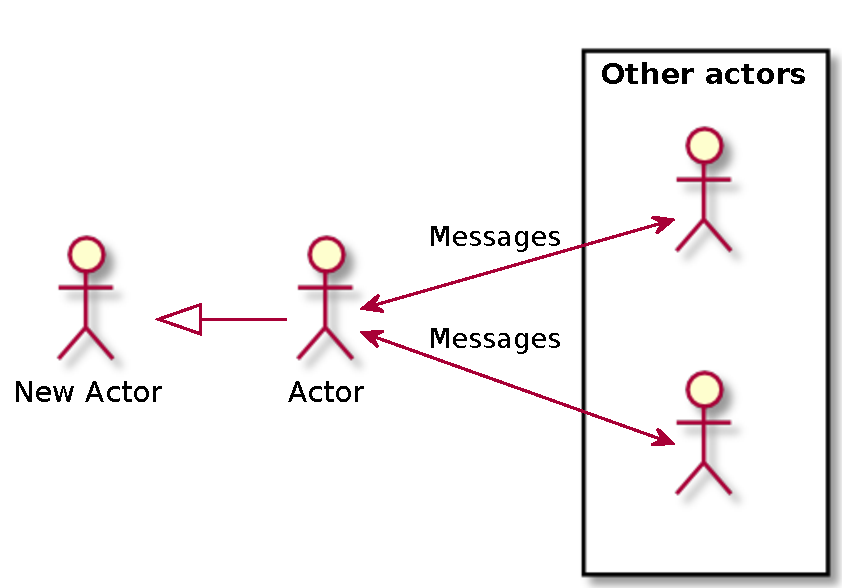
\includegraphics[width=0.6\textwidth]{cluster04/actor}
  \caption{Actor模型简单示意图}
  \label{cluster:fig:actor}
\end{figure}

我们的系统中在实现中采用了基于Scala语言的Actor库Akka\footnote{网址
  为:http://akka.io}。接下来我们需要对计算任务进行分割,以便使用\texttt{Actor}模
型来并行地进行计算。

对于一个文档集合,我们将计算其中两两文档之间的结构相似度的任务映射到几何平面上,
相当于计算一个正方形按对角线分割的一个三角形区域,三角形区域的某个点$(i, j)$表示
文档$D_i$和$D_j$之间的结构相似度。我们用等距的水平和垂直线分割这个三角形区域,把
整个任务分成许多子任务,如\reffig{cluster:fig:triangle}所示。计算的时候,建立一个
主\texttt{Actor}和一个监听\texttt{Actor},主\texttt{Actor}负责根据配置创造新
的\texttt{Actor},并使用调度器(我们使用的是简单的\texttt{RoundRobin}调度算法)来
向每个\texttt{Actor}动态分配任务。当主\texttt{Actor}创建的\texttt{Actor}都已经计
算完毕,并且没有剩下的计算任务可以分配的时候,主\texttt{Actor}负责向监
听\texttt{Actor}发送消息,告知任务完成,监听\texttt{Actor}则负责将整个系统关闭。
这样一个计算的模式我们后面还会用到,因此我们将其做了封装,隐藏了底层
的\texttt{Actor}模型的实现细节,便于后续的使用。
\begin{figure}
  \centering
  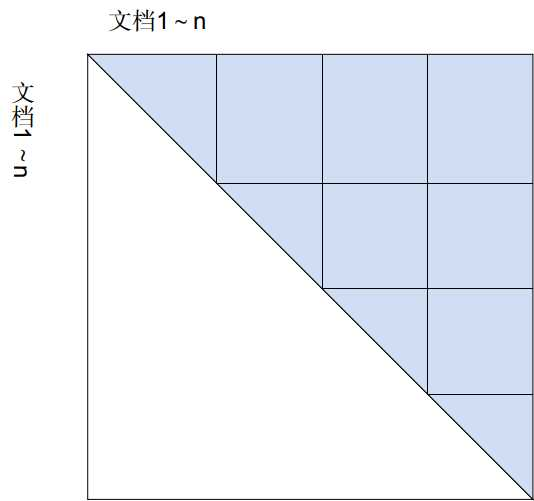
\includegraphics[width=0.45\textwidth]{cluster04/triangle}
  \caption{任务分割示意图}
  \label{cluster:fig:triangle}
\end{figure}

由于使用了并行的计算方式,在有较多计算资源的计算机上,计算网页结构相似度的模块可
以较快地完成。

\subsection{计算方式优化}
在原始的实现中,我们忽略了在先序遍历DOM Tree的时候保存下来的节点的深度信息。实际
上,不同深度的节点对模板的影响是不一样的,离根节点越近,即深度越小的节点,其成为
模板的一部分的可能性就越大;反之,其成为模板一部分的概率就越小。因此,我们可以将
最长公共子序列的计算方式进行扩充,根据节点的深度信息给表格$T$的每个点进行加权,设
加权函数为$f(depth)$,则修改后的算法的递推式变为:
\begin{eqnarray}
  t(i)(j) =
  \begin{cases}
    0 & i = 0,\: j = 0\\
    t(i-1)(j-1) + f(x_i.depth) & i,\: j > 0, x_i=y_j\\
    \max(t(i)(j-1), t(i-1)(j)) & i, j > 0,\: x_i \ne y_j
  \end{cases}
\end{eqnarray}

这样做的好处是将一些深度很大的节点的权重减小,使得算法更倾向于将深度更小的节点进
行匹配,因此可以得到更好的匹配效果。修改后的算法得到的$t(len_1)(len_2)$的值并不是
简单意义上最长公共子序列的长度,我们将其记为$|elcs(S_1,S_2)|$,相应地,我们需要修
改用于计算文档$D_1$和$D_2$的相似度的公式:
\[
Sim(D_1,D_2)=\frac{|elcs(S_1,S_2)|}{\max(\sum\limits_{n\in
    S_1}{f(n.depth)},\sum\limits_{n\in S_2}{f(n.depth)})}
\]
\section{聚类算法实现}
\label{sec:clusteralgo}
聚类的目的是为了将有明显差异的模板生成的网页分开,因此,我们可以认为需要分开的网
页的结构相似度是比较低的。同时,在聚类之前我们并不清楚这些网页是由几种不同模板生
成的,因此不能采用需要预先设置类别个数的聚类方法,比如$K-means$。在我们的系统中,
为了实现高效的自动的聚类,我们采用了一个简单的自底向上的凝聚层次聚类算法。

算法本身很简单:初始时,让每个文档实例都单独为一类,之后不断迭代,每次选择距离最
近的两个类合并,直到任意两个类的距离都大于阈值时程序退出。这个聚类算法的结束条件
由阈值决定,无需实现设定类的个数。具体的算法实现如伪代
码~\ref{cluster:algo:clustering}所示。这里说明一下类中心点的更新方法:由于我们只
有文档之间的结构相似度作为聚类的标准,每个文档实例本身没有合适的可度量的表示方法,
不能求平均,因此类似$K-medoids$,我们选择到类中所有点距离之和最短的点作为类的中心
点。
\begin{algorithm}
  \caption{简单的自底向上的凝聚层次聚类算法}
  \label{cluster:algo:clustering}
  \begin{algorithmic}[1]
    \Require 所有的文档实例$instances$,已经存储下来的计算好的距离$distances$和
    聚类的阈值$threshold$
    \Ensure 聚类后的类的集合$clusters$
    \Function{aggloClustering}{$instances, distances, threshold$}
    \State $//$初始化类的集合为空
    \State $clusters := Collection.empty$
    \State $//$每一个文档实例单独看成一个聚类,加入到类集合中
    \For{$inst \gets instances$}
    \State $c := \mathbf{new}~Cluster(inst)$
    \State $clusters.add(c)$
    \EndFor
    \State $//$不停迭代,直到最接近的两个聚类的距离大于设定的阈值为止
    \While{true}
    \State $//$从全部聚类中取出两个距离最近类
    \State $(c_1,c_2) := getMinDistanceClusterPair(clusters)$
    \State $//$如果距离已经大于预先设定的阈值,退出
    \If{$distances(c_1,c_2) > threshold$}
    \State $\mathbf{break;}$
    \EndIf
    \State $//$合并两个类,更新类中心,更新类集合
    \State $c_{merge} := mergeCluster(c_1,c_2)$
    \State $clusters.remove(c_1);clusters.remove(c_2);$
    \State $clusters.add(c_{merge})$
    \EndWhile
    \State $//$返回聚类结果
    \State \Return $clusters$
    \EndFunction
  \end{algorithmic}
\end{algorithm}

聚类过程可以用\reffig{cluser:fig:aggloclustering}简单表示。这个例子中一开始有5个
类,每一步选择最近的两个类进行一次凝聚,最后聚成两个类。
\begin{figure}
  \centering
  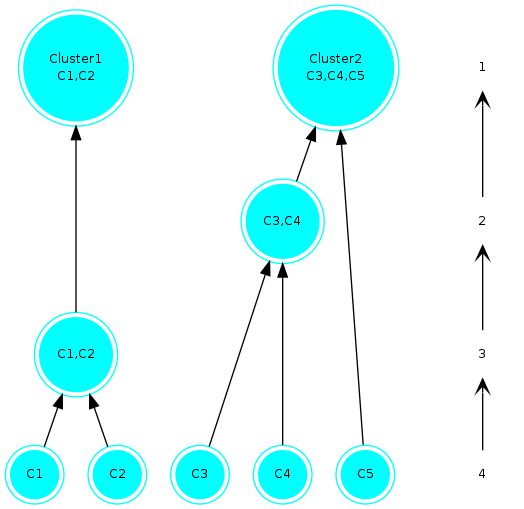
\includegraphics[width=0.6\textwidth]{cluster04/aggloclustering}
  \caption{简单层次聚类方法图示}
  \label{cluser:fig:aggloclustering}
\end{figure}
\section{本章总结}
\label{sec:summarycluster}
这一章我们先介绍了传统的最长公共子序列的计算方法,然后分别介绍了如何对原有的算法
进行优化,包括空间、时间和计算方式上的优化。在时间优化的部分,我们引入
了\texttt{Actor}作为我们并行计算的模型,并在系统中用\texttt{Actor}模型简单实现了
我们文档结构相似度计算的模块。最后我们介绍了我们采用的凝聚层次聚类算法。通过设置
合适的阈值,我们可以通过聚类算法将差异很大的模板生成的网页成功分开,之后这些聚类
将作为下一个模块的输入,进行模板的提取。
%%% Local Variables: 
%%% mode: latex
%%% TeX-master: "../main"
%%% End: 
